\documentclass[pdftex,12pt, oneside]{article}

%\usepackage[paperwidth=8.5in, paperheight=13in]{geometry} % Folio
\usepackage[paperwidth=8.27in, paperheight=11.69in]{geometry} % A4

\usepackage{makeidx}         % allows index generation
\usepackage{graphicx}        % standard LaTeX graphics tool
                             % when including figure files
\usepackage[bottom]{footmisc}% places footnotes at page bottom
\usepackage[english]{babel}
\usepackage{enumerate}
\usepackage{paralist}
\usepackage{float}
\usepackage{gensymb}  
\usepackage{listings}
\usepackage{color}
\usepackage{mathtools} % atau \usepackage{amsmath}
\renewcommand{\baselinestretch}{1.5}

\newcommand{\HRule}{\rule{\linewidth}{0.5mm}}

\definecolor{codegreen}{rgb}{0,0.6,0}
\definecolor{codegray}{rgb}{0.5,0.5,0.5}
\definecolor{codepurple}{rgb}{0.58,0,0.82}
\definecolor{backcolor}{rgb}{0.95,0.95,0.92}

\lstdefinestyle{mystyle}{
  backgroundcolor=\color{backcolor},
  commentstyle=\color{codegreen},
  keywordstyle=\color{magenta},
  stringstyle=\color{codepurple},
  basicstyle=\footnotesize,
  breakatwhitespace=false,
  breaklines=true,
  captionpos=b,
  keepspaces=true,
  numbers=left,
  numbersep=5pt,
  showspaces=false,
  showstringspaces=false,
  showtabs=false,
  tabsize=2
}

\lstset{style=mystyle}


\begin{document}
\sloppy % biar section ga melebar melewati kertas

\begin{center}
{\large RANCANGAN SISTEM \textit{WEB SERVICES} SEBAGAI CARA KOMUNIKASI DENGAN TEMPAT PEMBAYARAN DALAM PENCATATAN PEMBAYARAN PAJAK BUMI DAN BANGUNAN PERDESAAN DAN PERKOTAAN DI KABUPATEN BREBES.}
\\[1cm]
DD MMM 2016\\
Priyanto Tamami, S.Kom.
\end{center}

%\frontmatter%%%%%%%%%%%%%%%%%%%%%%%%%%%%%%%%%%%%%%%%%%%%%%%%%%%%%%


%%%%%%%%%%%%%%%%%%%%%%%%%%%%%%%%%%%%%%%%%%%%%%%%%%%%%%%%%%%%%%%%%%%%%%

\section{TUJUAN SISTEM}

Tujuan dari dibangunnya sistem \textit{web services} ini adalah mempermudah pencatatan transaksi pembayaran yang terjadi melalui Bank agar tersimpan pada basis data Sistem Manajemen Informasi Objek Pajak PBB-P2.


\section{PEMODELAN SISTEM}

Sistem akan dimodelkan sebagai bentuk \textit{web services} yang menerima 3 (tiga) bentuk masukan, yaitu untuk melakukan \textit{inquiry}, pencatatan pembayaran, dan \textit{reversal}.

Karena perangkat pemrograman yang digunakan nantinya mendukung pemrograman berorientasi objek, maka akan lebih mudah apabila pendekatan pemodelan menggunakan \textit{Unified Modeling Language} (UML). Bentuk-bentuk diagram yang akan digunakan adalah sebagai berikut :

\begin{enumerate}
  \item Diagram \textit{Use-Case}
  
  Diagram ini akan mengilustrasikan gambaran utuh sebuah sistem yang berinteraksi dengan pengguna.
  
  \item Diagram \textit{Activity}
  
  Diagram ini akan mengilustrasikan aktifitas dari tiap objek yang saling berinteraksi membentuk sebuah sistem yang menerima masukkan, memprosesnya, dan kemudian menghasilkan sebuah keluaran yang dibutuhkan.
  
  \item Diagram \textit{Class}
  
  Diagram ini akan mengilustrasikan kelas-kelas pembentuk sistem berdasarkan objek-objek yang teridentifikasi sebelumnya.
  
  \item Diagram \textit{Sequence}
  
  Diagram ini akan mengilustrasikan alur interaksi dari tiap kelas berdasarkan skenario tertentu.
  
\end{enumerate}

Lebih detail mengenai diagram-diagram tersebut akan dijelaskan sebagai berikut.


\subsection{Diagram \textit{Use-Case}}

Diagram \textit{Use-Case} ini akan menjelaskan gambaran menyeluruh atau gambaran besar aktifitas antara pengguna dengan sistem yang dibangun. Diagram \textit{Use-Case} pada sistem ini seperti terlihat pada gambar \ref{fig:uml-use-case} :

\begin{figure}[H]
  \centering
  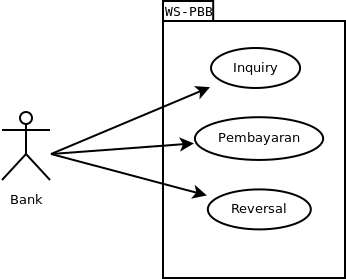
\includegraphics[width=0.5\textwidth]{./resources/uml/uml-use-case}
  \caption{Diagram \textit{Use-Case} Sistem \textit{Web Services} Pencatatan Pembayaran PBB-P2}
  \label{fig:uml-use-case}
\end{figure}

Yang menjadi aktor disini adalah Bank dalam artian \textit{client} yang akan melakukan akses ke sistem \textit{web services} pencatatan pembayaran Pajak Bumi dan Bangunan Perdesaan dan Perkotaan (PBB-P2).

Akses yang dapat dilakukan oleh \textit{client} ada 3 (tiga) skenario, yaitu \textit{Inquiry}, Pembayaran, dan \textit{Reversal}

\textit{Inquiry} ini adalah permintaan informasi PBB-P2 Terhutang oleh \textit{client} ke \textit{server web services}. Skenario Pembayaran adalah permintaan dari \textit{client} ke \textit{server web services} untuk melakukan pencatatan pembayaran PBB-P2 berdasarkan Nomor Objek Pajak (NOP) dan Tahun Pajak yang akan dicatatkan pembayarannya. Sedangkan skenario \textit{reversal} adalah permintaan oleh \textit{client} ke \textit{server web services} untuk melakukan pembatalan pencatatan pembayaran yang telah dilakukan.

\subsection{Diagram \textit{Activity}}

Diagram \textit{Activity} ini akan menggambarkan alur dari tiap skenario yang terdapat pada diagram \textit{use-case}. Diagramnya akan dijelaskan lebih lanjut pada bagian berikut.

\subsubsection{Diagram \textit{Activity} Untuk Skenario \textit{Inquiry}}

Diagram \textit{activity} untuk skenario \textit{inquiry} ini akan menjelaskan alur proses dari skenario \textit{inquiry} atau skenario permintaan data oleh \textit{client} berupa informasi tagihan PBB-P2. Diagram \textit{activity} untuk skenario \textit{inquiry} ini seperti terlihat pada gambar \ref{fig:uml-act-inquiry} :

\begin{figure}[H]
  \centering
  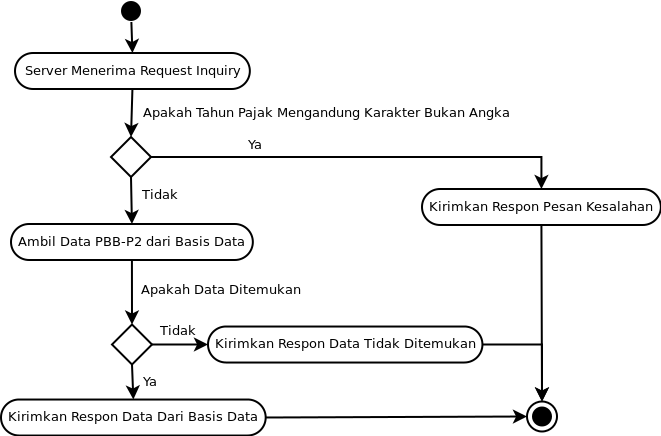
\includegraphics[width=0.8\textwidth]{./resources/uml/uml-act-inquiry}
  \caption{Diagram \textit{Activity} Untuk Skenario \textit{Inquiry}}
  \label{fig:uml-act-inquiry}
\end{figure}

Pada skenario \textit{inquiry} ini, awalnya \textit{server} akan menerima \textit{request inquiry} dari \textit{client}, kemudian \textit{server} melakukan pemeriksaan apakah tahun pajak yang menjadi parameter masukkan permintaan data mengandung karakter selain angka atau tidak, bila mengandung angka, maka \textit{server} akan mengirimkan respon kesalahan ke \textit{client} bahwa tahun pajak yang diminta mengandung karakter bukan angka.

Bila tahun pajak tidak mengandung karaketer bukan angka, maka \textit{server} aplikasi \textit{web services} akan melakukan pengambilan data ke \textit{server} basis data dan dilakukan pengecekan, apakah data yang diminta ada atau tidak, bila tidak ada \textit{server} akan mengirimkan respon kesalahan ke \textit{client} bahwa data yang diminta tidak ditemukan. Namun bila data ditemukan maka \textit{server} akan mengirimkan respon ke \textit{client} data yang diminta.

\subsubsection{Diagram \textit{Activity} Untuk Skenario Pencatatan Pembayaran}

Diagram \textit{activity} untuk skenario pencatatan pembayaran akan menjelaskan alur aktifitas pada saat \textit{client} melakukan \textit{request} pencatatan pembayaran ke \textit{server}. Diagram \textit{activity} untuk skenario ini seperti terlihat pada gambar \ref{fig:uml-act-bayar} :

\begin{figure}[H]
  \centering
  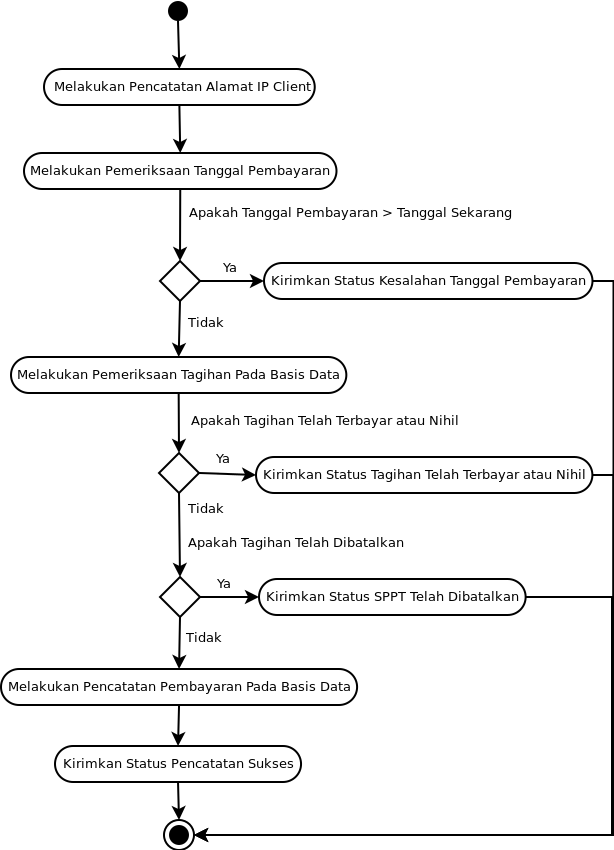
\includegraphics[width=0.8\textwidth]{./resources/uml/uml-act-bayar}
  \caption{Diagram \textit{Activity} Untuk Skenario Pencatatan Pembayaran}
  \label{fig:uml-act-bayar}
\end{figure}

Pertama yang ditangani oleh \textit{server} dari \textit{client} adalah melakukan pencatatan alamat IP \textit{client} untuk keperluan audit. 

Kemudian melakukan pemeriksaan terhadap parameter tanggal pembayaran, bila tanggal pembayaran lebih dari tanggal saat ini, maka \textit{server} akan mengirimkan respon kesalahan ke \textit{client} karena tidak mungkin tanggal pembayaran terjadi setelah tanggal pencatatan ke SISMIOP.

Selanjutnya adalah melakukan pemeriksaan tagihan pada basis data sesuai parameter yang dikirimkan oleh \textit{client}. Apabila tagihan telah terbayar, atau jumlah tagihan nihil, atau tagihan telah dibatalkan, maka \textit{server} akan mengirimkan respon informasi ke \textit{client} bahwa nomor objek pajak untuk tahun pajak yang diminta telah terbayar, nihil, atau telah dibatalkan.

Langkah setelah melewati serangkaian pemeriksaan parameter tersebut adalah melakukan pencatatan pembayaran pada basis data dan mengirimkan respon informasi ke \textit{client} bahwa pencatatan pembayaran pada basis data telah sukses dan selesai.

\subsubsection{Diagram \textit{Activity} Untuk Skenario \textit{Reversal}}

Diagram \textit{activity} untuk \textit{reversal} akan menggambarkan rinci dari alur proses \textit{reversal} terjadi. Diagram \textit{activity} untuk skenario \textit{reversal} ini seperti terlihat pada gambar \ref{fig:uml-act-reversal} :

\begin{figure}[H]
  \centering
  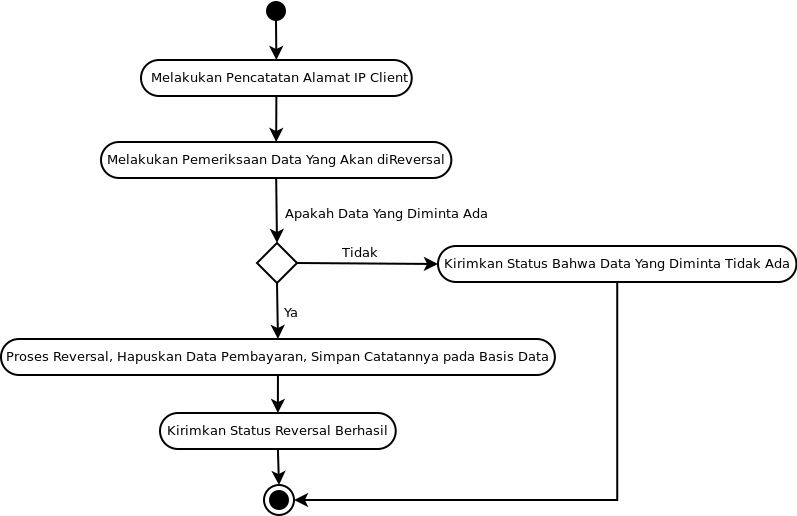
\includegraphics[width=0.5\textwidth]{./resources/uml/uml-act-reversal}
  \caption{Diagram \textit{Activity} Untuk Skenario \textit{Reversal}}
  \label{fig:uml-act-reversal}
\end{figure}

Seperti pada skenario pembayaran, karena transaksi yang dilakukan pada kasus ini akan merubah isi dari basis data, maka hal pertama yang dilakukan adalah mencatat alamat IP dari \textit{client}.

Kemudian melakukan pemeriksaan pada basis data apakah data yang diminta untuk dilakukan \textit{reversal} berdasarkan parameter-parameter yang dikirimkan ada pada basis data atau tidak, bila tidak ada maka \textit{server} akan mengirimkan respon kesalahan bahwa data yang diminta tidak ada.

Bila data yang diminta ada pada basis data, maka proses \textit{reversal} dilakukan, yaitu dengan menghapuskan data pembayaran dan merubah \textit{flag} status pembayaran pada tabel sppt, dan menyimpan catatan penghapusan data pembayaran pada basis data. Terakhir mengirimkan respon ke \textit{client} bahwa proses \textit{reversal} telah selesai dilakukan.

\subsection{Diagram \textit{Class}}

Pada diagram \textit{class} akan digambarkan hubungan dari tiap kelas hasil implementasi dari objek-objek yang tergambar pada diagram \textit{activity}, namun ada beberapa kelas-kelas yang memang terbentuk karena lingkungan \textit{framework} mengharuskan seperti itu.

Diagram \textit{class} untuk sistem ini seperti terlihat pada gambar \ref{fig:uml-class} :

\begin{figure}[H]
  \centering
  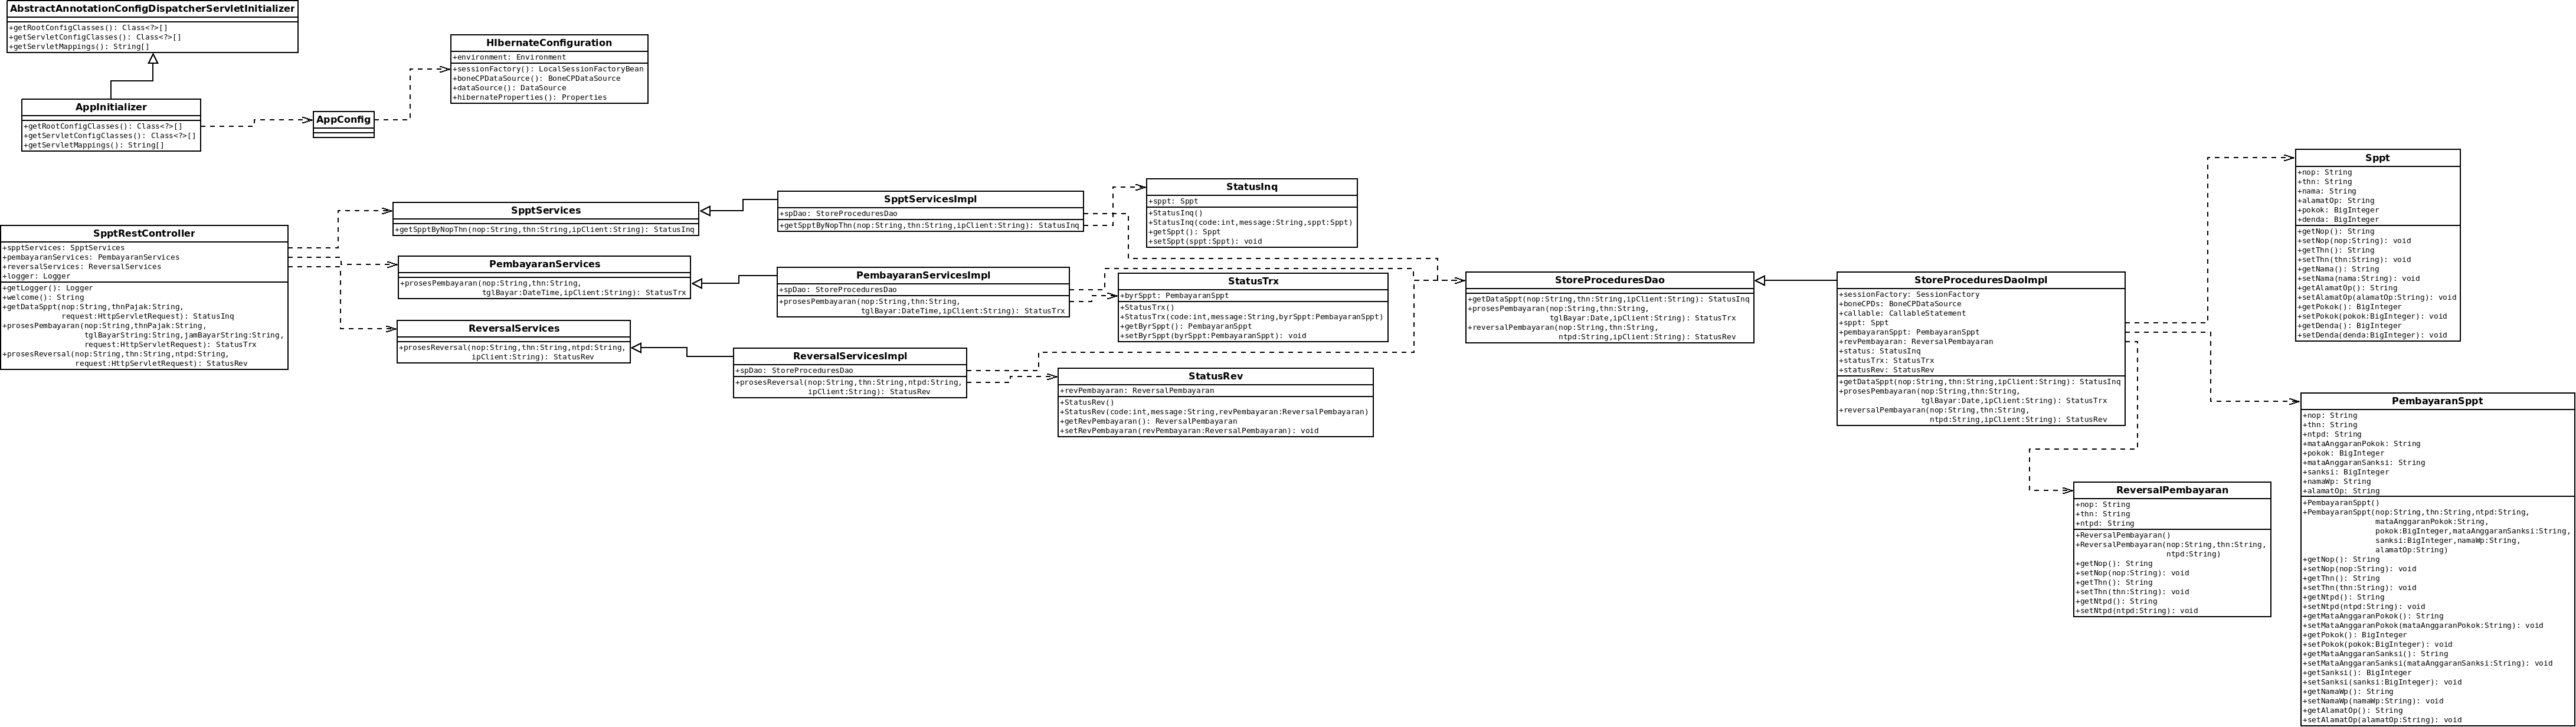
\includegraphics[width=1\textwidth]{./resources/uml/uml-class}
  \caption{Diagram \textit{Class}}
  \label{fig:uml-class}
\end{figure}

Kelas-kelas yang merupakan tuntutan dari \textit{framework} Spring adalah kelas AppInitializer dan AppConfig. AppInitializer adalah kelas awal yang mewarisi \textit{interface} AbstractAnnotationConfigDispatcherServletInitializer milik Spring yang akan dipanggil pada saat awal aplikasi web akan dijalankan.

Sedangkan kelas AppConfig adalah kelas yang akan menampung konfigurasi aplikasi web nantinya, termasuk disana adalah pemanggilan kelas konfigurasi lainnya, yaitu HibernateConfig yang bertugas melakukan konfigurasi terhadap komunikasi yang terjadi antara aplikasi dengan \textit{server} basis data.

Titik awal dari setiap \textit{request} yang masuk ke \textit{server} akan melalui kelas SpptRestController, dari kelas ini nantinya akan diteruskan ke kelas-kelas \textit{services} yang melayani, seperti kelas SpptServiceImpl, PembayaranServicesImpl, dan ReversalServicesImpl.

Kelas-kelas \textit{services} ini akan bermuara pada satu kelas \textit{Data Access Object} (DAO) yaitu kelas StoreProceduresDaoImpl. Kelas inilah yang nantinya melakukan akses ke \textit{server} basis data, dan mengembalikannya dalam bentuk objek-objek atau kelas-kelas berikut : Kelas Sppt, untuk menampung informasi tagihan yang tercatat dalam basis data; kelas PembayaranSppt, untuk menampung informasi pencatatan pembayaran yang telah dilakukan dan sukses; yang terakhir adalah kelas ReversalPembayaran, yaitu untuk menampung transaksi \textit{reversal} yang telah sukses.

\subsection{Diagram \textit{Sequence}}

Diagram \textit{sequence} ini akan menggambarkan interaksi antar kelas untuk tiap alur skenario yang terjadi. Hasil skenario yang terdata adalah sebagai berikut :

\subsubsection{Diagram \textit{Sequence} Untuk Skenario Konfigurasi \textit{Spring Framework}}

Diagram \textit{sequence} untuk skenario konfigurasi \textit{Spring Framework} akan menjelaskan alur yang terjadi saat \textit{container} melakukan inisialisasi sistem untuk siap menerima \textit{request} dari \textit{client}. Diagram ini seperti terlihat pada gambar \ref{fig:uml-seq--konf} :

\begin{figure}[H]
  \centering
  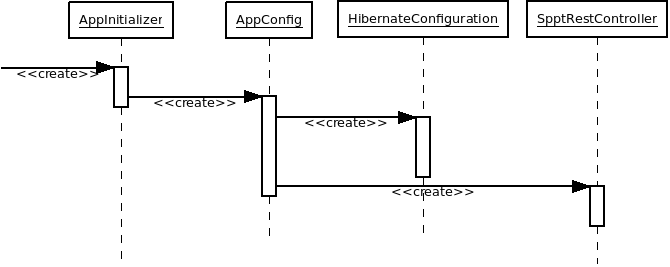
\includegraphics[width=0.5\textwidth]{./resources/uml/uml-seq-konf}
  \caption{Diagram \textit{Sequence} Untuk Skenario Konfigurasi \textit{Spring Framework}}
  \label{fig:uml-seq-konf}
\end{figure}

Pada saat sistem sudah di \textit{deploy} pada \textit{container}, maka kelas awal yang diperiksa dan dieksekusi adalah kelas AppInitializer, kemudian kelas AppInitializer ini akan melakukan pembentukan instan kelas AppConfig, kemudian kelas AppConfig akan melakukan eksekusi terhadap kelas HibernateConfiguration sebagai penghubung dengan sistem basis data, dan kelas SpptRestController yang melakukan tugasnya sebagai pengontrol tiap \textit{request} yang diterima, dan diteruskan ke bagian-bagian yang menangani.

\subsubsection{Diagram \textit{Sequence} Untuk Skenario \textit{Inquiry} Gagal Karena Tahun Pajak Bukan Angka}

Diagram \textit{sequence} untuk skenario ini akan menjelaskan alur eksekusi dari awal \textit{request} diterima, sampai kepada kondisi dimana \textit{request} gagal untuk diproses karena parameter tahun pajak memiliki karakter bukan angka. Diagram untuk skenario ini seperti terlihat pada gambar \ref{fig:uml-seq-inq-thn-not-valid} :

\begin{figure}[H]
  \centering
  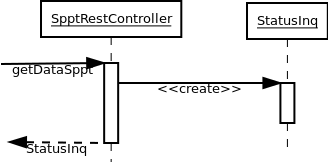
\includegraphics[width=0.5\textwidth]{./resources/uml/uml-seq-inq-thn-not-valid}
  \caption{Diagram \textit{Sequence} Untuk Skenario \textit{Inquiry} Yang Gagal Karena Tahun Pajak Mengandung Karakter Bukan Angka}
  \label{fig:uml-seq-inq-thn-not-valid}
\end{figure}

Setiap \textit{request inquiry} yang masuk ke \textit{server} akan melalui \textit{method} getDataSppt milik kelas SpptRestController, kemudian pada \textit{method} getDataSppt ini akan dilakukan pemeriksaan terhadap parameter tahun pajak yang diinginkan oleh \textit{client}.

Saat ditemukan bahwa parameter tahun pajak mengandung karakter bukan angka, maka akan dibuat instan dari kelas StatusInq sebagai bahan respon terhadap \textit{client} bahwa \textit{request} yang diminta tidak dapat diproses.

\subsubsection{Diagram \textit{Sequence} Untuk Skenario \textit{Inquiry} Gagal Karena Data Tidak Ditemukan}

Diagram \textit{sequence} ini akan menggambarkan alur komunikasi \textit{inquiry} yang gagal karena data Nomor objek Pajak (NOP) untuk tahun pajak yang diminta tidak ada pada basis data. Diagramnya terlihat seperti pada gambar \ref{fig:uml-seq-inq-not-any} :

\begin{figure}[H]
  \centering
  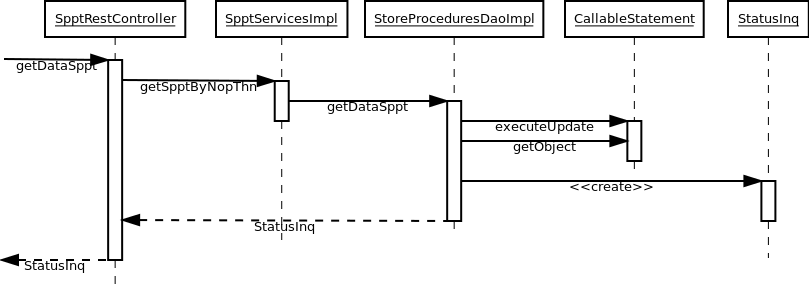
\includegraphics[width=0.8\textwidth]{./resources/uml/uml-seq-inq-not-any}
  \caption{Diagram \textit{Sequence} Untuk Skenario \textit{Inquiry} Yang Gagal Karena Data Tidak Ditemukan Dalam Basis Data}
  \label{fig:uml-seq-inq-not-any}
\end{figure}

\textit{Request} yang masuk ke \textit{server} terhadap \textit{inquiry} akan datang ke \textit{method} getDataSppt milik kelas SpptRestController, berdasarkan parameter Nomor Objek Pajak (NOP) dan tahun pajak, \textit{method} ini akan memanggil \textit{method} getSpptByNopThn milik kelas SpptServicesImpl, dari \textit{method} getSpptByNopThn milik kelas SpptServicesImpl akan memanggil \textit{method} getDataSppt milik kelas StoreProceduresDaoImpl.

Selanjutnya di dalam \textit{method} getDataSppt milik kelas StoreProceduresDaoImpl melakukan eksekusi \textit{store procedure} dengan memanggil \textit{method} executeUpdate milik kelas CallableStatement, kemudian mengambil hasil dari pemanggilan \textit{store procedure} pada basis data dengan \textit{method} getObject.

Namun pada saat pemanggilan \textit{method} getObject, data yang diminta tidak ada dalam basis data, sehingga kelas StoreProceduresDaoImpl akan membuat instan dari kelas StatusInq yang berisi informasi bahwa objek pajak untuk tahun pajak yang diinginkan tidak ada pada basis data. Kemudian instan kelas StatusInq ini dikembalikan ke kelas SpptRestController sebagai bahan respon ke \textit{client}.

\subsubsection{Diagram \textit{Sequence} Untuk Skenario \textit{Inquiry} Gagal Karena Kesalahan Server}

Diagram ini akan menjelaskan alur komunikasi data antar kelas bila ada kesalahan proses saat melakukan pemanggilan \textit{store procedure} pada \textit{server} basis data. Diagram \textit{sequence} untuk skenario ini seperti terlihat pada gambar \ref{fig:uml-seq-inq-db-error} :

\begin{figure}[H]
  \centering
  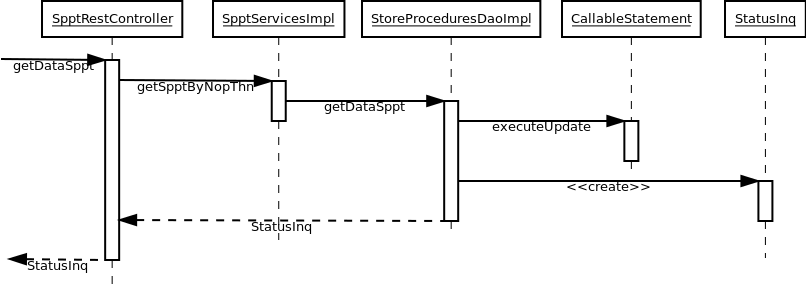
\includegraphics[width=0.8\textwidth]{./resources/uml/uml-seq-inq-db-error}
  \caption{Diagram \textit{Sequence} Untuk Skenario \textit{Inquiry} Yang Gagal Karena Kesalahan Komunikasi Antara \textit{Server} Aplikasi Dengan \textit{Server} Basis Data}
  \label{fig:uml-seq-inq-db-error}
\end{figure}

\textit{Request} yang masuk untuk skenario \textit{inquiry} akan diterima dan diproses oleh \textit{method} getDataSppt milik kelas SpptRestController. Dari \textit{method} ini, kemudian akan dipanggil \textit{method} getSpptByNopThn milik kelas SpptServicesImpl.

Dari \textit{method} getSpptByNopThn milik kelas SpptServicesImpl, kemudian memanggil \textit{method} getDataSppt milik kelas StoreProceduresDaoImpl, yang kemudian mencoba melakukan eksekusi \textit{store procedure} milik basis data dengan memanggil \textit{method} executeUpdate milik kelas CallableStatement, tetapi eksekusi ini karena beberapa hal yang tidak diketahui, hubungan komunikasi antara \textit{server} Aplikasi dengan \textit{server} basis data terputus, sehingga keluar \textit{exception} dan proses pengambilan atau \textit{inquiry} data tidak dapat diteruskan.

Sampai sini, \textit{method} getDataSppt milik kelas StoreProceduresDaoImpl akan membuat instan dari kelas StatusInq yang berisi informasi kegagalan komunikasi ke \textit{server} basis data, hasil instan dari kelas StatusInq ini dikirimkan kembali ke kelas SpptRestController yang nantinya memberikan respon ke \textit{client} bahwa proses \textit{inquiry} gagal dilakukan.

\subsubsection{Diagram \textit{Sequence} Untuk Skenario \textit{Inquiry} Yang Sukses}

Diagram ini akan menjelaskan alur yang terjadi saat \textit{request inquiry} berhasil di respon sesuai data yang ada pada basis data. Diagram \textit{sequence} untuk skenario ini seperti terlihat pada gambar \ref{fig:uml-seq-inquiry} :

\begin{figure}[H]
  \centering
  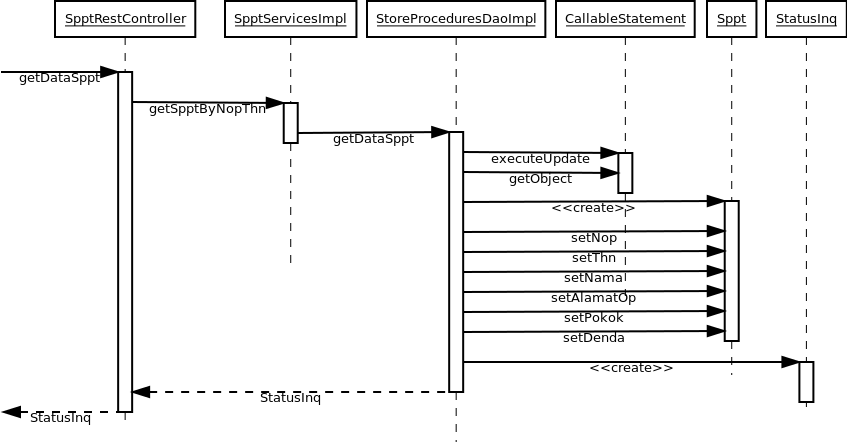
\includegraphics[width=1\textwidth]{./resources/uml/uml-seq-inquiry}
  \caption{Diagram \textit{Sequence} Untuk Skenario \textit{Inquiry} Yang Sukses}
  \label{fig:uml-seq-inquiry}
\end{figure}

Proses \textit{request inquiry} dari \textit{client} akan berawal dari \textit{method} getDataSppt milik kelas SpptRestController, kemudian memanggil \textit{method} getSpptByNopThn milik kelas SpptServicesImpl, dari \textit{method} ini kemudian memanggil \textit{method} getDataSppt milik kelas StoreProceduresDaoImpl yang kemudian melakukan eksekusi terhadap \textit{store procedures} milik basis data dengan memanggil \textit{method} executeUpdate milik kelas CallableStatement.

Untuk mendapatkan hasil dari pemanggilan \textit{store procedures} milik basis data, maka perlu dilakukan pemanggilan \textit{method} getObject milik kelas CallableStatement, yang hasilnya dimasukkan sebagai parameter pembentuk kelas Sppt.

Langkah terakhir adalah membungkus instan kelas Sppt yang telah terisi data dari basis data dengan kelas StatusInq, kemudian instan dari kelas ini dikembalikan ke kelas SpptRestController yang akhirnya dikirimkan ke \textit{client} sebagai respon \textit{inquiry}.

\subsubsection{Diagram \textit{Sequence} Untuk Skenario Transaksi Pembayaran Gagal Karena Jam Pembayaran Melebihi Jam Pencatatan}

Diagram ini akan menjelaskan alur komunikasi antar kelas pada saat ada \textit{request} pencatatan transaksi pembayaran tetapi gagal karena jam pada saat pembayaran melebihi jam pada saat pencatatan di basis data, karena tidak mungkin transaksi yang terjadi tercatat lebih dulu sebelum terjadinya pembayaran. Diagram \textit{sequence} untuk skenario ini seperti terlihat pada gambar \ref{fig:uml-seq-trx-tgl-bayar-error} :

\begin{figure}[H]
  \centering
  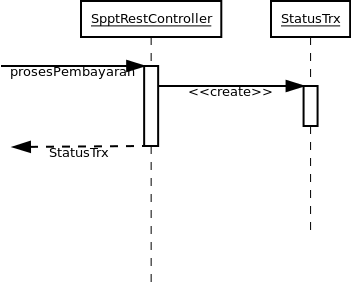
\includegraphics[width=0.5\textwidth]{./resources/uml/uml-seq-trx-tgl-bayar-error}
  \caption{Diagram \textit{Sequence} Untuk Skenario Transaksi Pembayaran Yang Gagal Karena Jam Pembayaran Melebihi Jam Pencatatan}
  \label{fig:uml-seq-trx-tgl-bayar-error}
\end{figure}

\textit{Request} yang datang dari \textit{client} akan langsung memanggil \textit{method} prosesPembayaran milik kelas SpptRestController. Di dalam \textit{method} ini, terdapat pemeriksaan parameter tanggal pembayaran yang apabila parameter tanggal pembayaran berisi tanggal yang melebihi tanggal saat ini, maka \textit{method} prosesPembayaran akan membentuk instan dari kelas StatusTrx, kemudian mengirimkan informasi kelas StatusTrx ini kepada \textit{client} bahwa tanggal dan jam pembayaran melebihi tanggal dan jam hari saat ini, sehingga proses pencatatan pembayaran tidak dapat dilakukan.

\subsubsection{Diagram \textit{Sequence} Untuk Skenario Transaksi Pembayaran Gagal Karena Tagihan Telah Terbayar Atau Nihil}

Diagram ini akan menceritakan alur komunikasi antar kelas untuk skenario transaksi pembayaran yang gagal karena tagihan telah terbayar atau memang tagihan untuk nomor objek pajak (NOP) dan tahun pajak tersebut nihil. Diagram \textit{sequence} untuk skenario ini seperti terlihat pada gambar \ref{fig:uml-seq-trx-nihil} :

\begin{figure}[H]
  \centering
  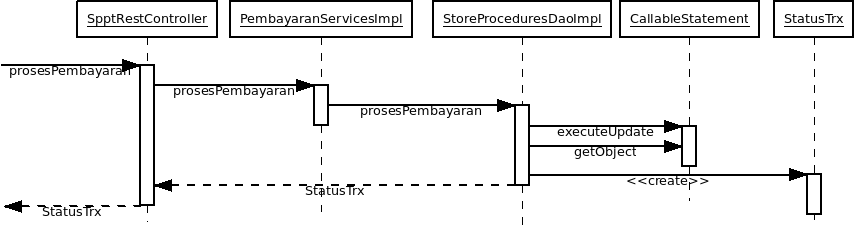
\includegraphics[width=0.8\textwidth]{./resources/uml/uml-seq-trx-nihil}
  \caption{Diagram \textit{Sequence} Untuk Skenario Transaksi Pembayaran Yang Gagak Karena Tagihan Telah Terbayar Atau Nihil}
  \label{fig:uml-seq-trx-nihil}
\end{figure}

\textit{Request client} akan langsung diarahkan ke \textit{method} prosesPembayaran milik kelas SpptRestController, kemudian \textit{method} ini akan memanggil \textit{method} prosesPembayaran milik kelas PembayaranServicesImpl, lalu \textit{method} ini akan memanggil \textit{method} prosesPembayaran milik kelas StoreProceduresDaoImpl.

Didalam \textit{method} prosesPembayaran milik kelas StoreProceduresDaoImpl, akan melakukan eksekusi terhadap \textit{store procedures} di sistem basis data dengan melakukan pemanggilan \textit{method} executeUpdate milik kelas CallableStatement, kemudian untuk mengambil hasil dari eksekusi \textit{store procedure}, dilakukan pemanggilan \textit{method} getObject milik kelas CallableStatement.

Karena datanya telah terbayar, atau tagihannya nihil, maka \textit{store procedure} akan memberikan keterangan kondisi ini yang hasilnya disimpan pada kelas StatusTrx dan dikembalikan ke kelas SpptRestController sebagai bahan respon ke \textit{client}.

\subsubsection{Diagram \textit{Sequence} Untuk Skenario Transaksi Pembayaran Gagal Karena Telah Dibatalkan}

Desain ini akan menjelaskan gambaran alur komunikasi antar kelas untuk skenario pencatatan transaksi pembayaran yang gagal karena tagihan untuk nomor objek pajak (NOP) dan tahun pajak yang diminta telah dibatalkan. Diagram \textit{Sequence} untuk skenario ini seperti pada gambar \ref{fig:uml-seq-trx-batal} :

\begin{figure}[H]
  \centering
  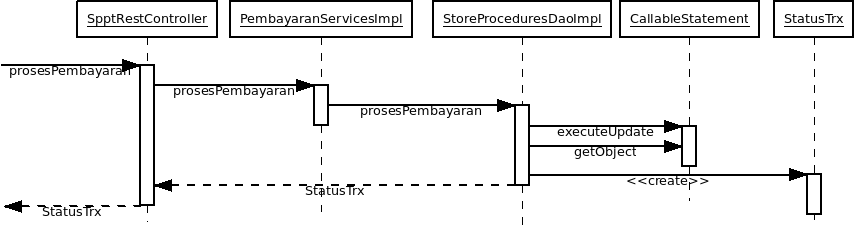
\includegraphics[width=1\textwidth]{./resources/uml/uml-seq-trx-batal}
  \caption{Diagram \textit{Sequence} Untuk Skenario Transaksi Pembayaran Yang Gagal Karena SPPT Telah Dibatalkan}
  \label{fig:uml-seq-trx-batal}
\end{figure}

Proses \textit{request} pencatatan pembayaran yang datang dari \textit{client} akan langsung masuk ke \textit{method} prosesPembayaran milik kelas SpptRestController, dari \textit{method} ini kemudian akan memanggil \textit{method} prosesPembayaran milik kelas PembayaranServicesImpl. 

Dalam \textit{method} prosesPembayaran pada kelas PembayaranServicesImpl, akan memanggil \textit{method} prosesPembayaran milik kelas StoreProceduresDaoImpl, dari \textit{method} ini kemudian akan melakukan eksekusi \textit{store procedure} milik basis data dengan memanggil \textit{method} executeUpdate milik kelas CallableStatement, untuk menampung hasil kembalian dari \textit{store procedure} maka digunakan \textit{method} getObject milik CallableStatement.

Hasil kembalian dari pemanggilan \textit{store procedure} memberikan informasi bahwa tagihan untuk nomor objek pajak (NOP) dan tahun pajak yang diminta telah dibatalkan, sehingga tidak ada pajak terhutang atas NOP dan tahun pajak tersebut.

Hasil dari kembalian \textit{store procedure} ini akan ditempatkan pada kelas StatusTrx yang dikembalikan ke kelas SpptRestController sebagai bahan respon ke \textit{client}

\subsubsection{Diagram \textit{Sequence} Untuk Skenario Transaksi Pembayaran Gagal Karena Kesalahan Server}

Diagram ini akan menjelaskan alur komunikasi untuk menangani skenario pencatatan transaksi pembayaran yang gagal karena ada kesalahan dengan komunikasi antara \textit{server} aplikasi dengan \textit{server} basis data. Diagram \textit{sequence} untuk menggambarkan skenario ini adalah seperti pada gambar \ref{fig:uml-seq-trx-db-error} :

\begin{figure}[H]
  \centering
  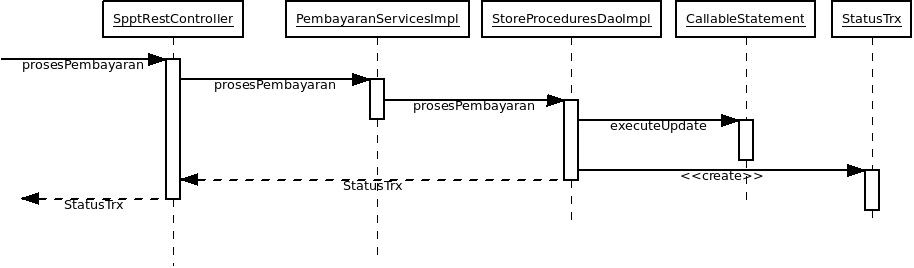
\includegraphics[width=1\textwidth]{./resources/uml/uml-seq-trx-db-error}
  \caption{Diagram \textit{Sequence} Untuk Skenario Transaksi Pembayaran Yang Gagal Karena Ada Kesalahan Di \textit{Server}}
  \label{fig:uml-seq-trx-db-error}
\end{figure}

\textit{Request} pencatatan transaksi pembayaran dari \textit{client} akan langsung ditangani oleh \textit{method} prosesPembayaran milik kelas SpptRestController. \textit{Method} ini kemudian akan melakukan pemanggilan ke \textit{method} prosesPembayaran milik kelas PembayaranServicesImpl, yang didalam \textit{method} ini pun akan memanggil \textit{method} prosesPembayaran dari kelas StoreProceduresDaoImpl.

Dari \textit{method} prosesPembayaran milik kelas StoreProceduresDaoImpl akan dieksekusi \textit{store procedure} milik basis data dengan memanggil \textit{method} executeUpdate milik kelas CallableStatement, namun karena ada beberapa kendala yang terjadi seperti putusnya koneksi jaringan, atau basis data dalam kondisi \textit{offline}, maka komunikasi antara \textit{server} aplikasi dengan \textit{server} basis data terganggu, sehingga munculah kesalahan disana.

Kesalahan muncul kemudian dicatatkan dalam instan kelas StatusTrx yang kemudian dikembalikan ke kelas SpptRestController sebagai bahan respon ke \textit{client}.

\subsubsection{Diagram \textit{Sequence} Untuk Skenario Transaksi Pembayaran Yang Sukses}

Diagram ini akan menggambarkan alur komunikasi antar kelas untuk menyelesaikan skenario pencatatan transaksi pembayaran yang sukses. Diagram \textit{sequence} untuk skenario ini seperti terlihat pada gambar \ref{fig:uml-seq-trx} :

\begin{figure}[H]
  \centering
  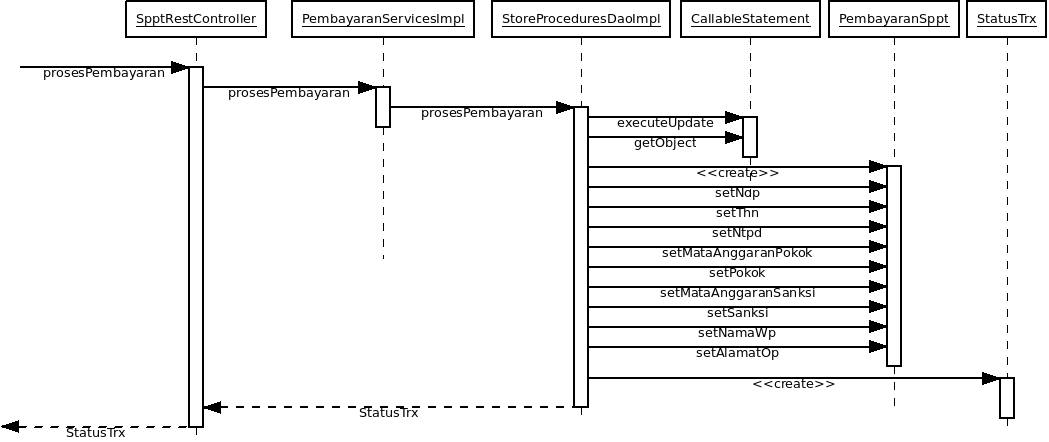
\includegraphics[width=1\textwidth]{./resources/uml/uml-seq-trx}
  \caption{Diagram \textit{Sequence} Untuk Skenario Transaksi Pembayaran Yang Sukses}
  \label{fig:uml-seq-trx}
\end{figure}

\textit{Request} dari \textit{client} akan langsung ditangani oleh \textit{method} prosesPembayaran milik kelas SpptRestController, \textit{method} ini kemudian melakukan pemanggilan \textit{method} prosesPembayaran milik kelas PembayaranServicesImpl, selanjutnya \textit{method} prosesPembayaran milik kelas PembayaranServicesImpl akan memanggil \textit{method} prosesPembayaran milik kelas StoreProceduresDaoImpl.

Dalam \textit{method} prosesPembayaran milik kelas StoreProceduresDaoImpl, ada beberapa kegiatan yang dilakukan, yaitu melakukan eksekusi \textit{store procedure} milik basis data dengan memanggil \textit{method} executeUpdate milik kelas CallableStatement, kemudian mengambil hasil dari pemanggilan \textit{store procedure} dengan \textit{method} getObject milik kelas CallableStatement pula, hasilnya disimpan dalam kelas PembayaranSppt.

Kemudian langkah selanjutnya adalah membuat instan dari kelas StatusTrx dan memasukan instan kelas PembayaranSppt didalamnya sebagai informasi ke \textit{client} bahwa proses pencatatan pembayaran telah dilakukan dengan sukses. Hasil instan kelas StatusTrx ini kemudian dikembalikan ke kelas SpptRestController sebagai bahan respon ke \textit{client}.

\subsubsection{Diagram \textit{Sequence} Untuk Skenario \textit{Reversal} Gagal Karena Data Yang Diminta Tidak Ada}

Diagram ini akan memberikan gambaran bagaimana arus komunikasi terjadi sehingga skenario proses reversal yang gagal karena data yang diminta tidak ada pada sistem basis data. 

\subsubsection{Diagram \textit{Sequence} Untuk Skenario \textit{Reversal} Gagal Karena Ada Data Pembayaran Yang Tercatat Ganda}
\subsubsection{Diagram \textit{Sequence} Untuk Skenario \textit{Reversal} Gagal Karena Kesalahan Server}
\subsubsection{Diagram \textit{Sequence} Untuk Skenario \textit{Reversal} Yang Sukses}


\section{AKTIVITAS PEMROSESAN DATA}

\begin{verbatim}
  Isinya :
    - output terpenting (goal)
    - identifikasi input 
    - alur pemrosesan data
  Arahnya ke unit testing
\end{verbatim}


\end{document}